% EuroS&P submission draft. Format: IEEE conference, A4, 13 body pages.
\documentclass[compsoc,conference,a4paper,10pt,times]{IEEEtran}
% Class options and IEEEtran.cls exactly as in the official EuroS&P 2027 template (zip sha256 5f074285...).
\IEEEoverridecommandlockouts
\usepackage{cite}
\usepackage{amsmath,amssymb,amsfonts}
\usepackage{graphicx,textcomp,xcolor}
\usepackage{booktabs,listings,tikz,multirow}
\usetikzlibrary{positioning,arrows.meta,fit,shapes.misc}
% Placeholders and notes. Red = something must be executed, built or decided.
% bold run-in heading (content macro; the class is not modified)
\newcommand{\para}[1]{\par\smallskip\noindent\textbf{#1.}\enspace}
\newcommand{\tool}{\textsc{BindCheck}}
% \TBD{} : a value we do not have yet (shown red)
\DeclareRobustCommand{\TBD}{\textcolor{red}{\textbf{TBD}}}
% \TODO{ID}{what must be done} : ID matches paper/eurosp/TODO.md
\DeclareRobustCommand{\TODO}[2]{\textcolor{red}{[\textbf{#1}: #2]}}
% \DEMO{text}: a strong final-style sentence whose values are expected, not yet measured (red).
\DeclareRobustCommand{\DEMO}[1]{\textcolor{red}{#1}}
\newcommand{\Pone}{P1}\newcommand{\Ptwo}{P2}\newcommand{\Pthree}{P3}\newcommand{\Pfour}{P4}\newcommand{\Pfive}{P5}
\newcommand{\finding}[1]{\par\smallskip\noindent\fbox{\parbox{\dimexpr\columnwidth-2\fboxsep-2\fboxrule}{\small\textbf{Takeaway.} #1}}\par\smallskip}
\lstset{basicstyle=\ttfamily\scriptsize,columns=fullflexible,breaklines=true,frame=tb,numbers=none,xleftmargin=2pt}

\usepackage[colorlinks=true,urlcolor=black]{hyperref}
\begin{document}
\title{\TODO{W1}{title}\thanks{NB: appendices, if any, did not benefit from peer review.}}
\author{\IEEEauthorblockN{Anonymous submission}}
\maketitle
\begin{abstract}Smart contracts accept zero-knowledge (ZK) proofs as permission to release
funds, mint credentials, and settle state. A proof certifies only a
statement, yet the contract's action can depend on values the statement never
fixed, such as a recipient taken from calldata. Anyone who observes a valid
proof can then redirect or repeat the effect. We call these \emph{binding
flaws}. Two such failures at the proof-to-contract boundary lost about
\$7.3M in 2025--2026, including \$2.28M drained from Aztec Connect. We define
binding as a relation between a \emph{statement ledger} and an \emph{effect
ledger} under the application's intended policy, and classify its violations
into five patterns that mirror classic signature misuse. In 8,578 public
audit reports we find 87 core binding flaws across 43 project families; 78\%
of those with a severity rating are Critical or High. Existing tools miss
them: Slither, Mythril, circomspect, Picus and generic fuzzing find none of
the audited flaws they could analyze, because the specification lives between
the circuit and the contract. We present \tool{}, which drives an LLM through
an explicit ledger procedure with deterministic analyses, per-proof-system
knowledge and a second look at every verdict, and attaches to each warning
the attack tests it ran on a local chain. A first version found 6 of 22
audited test-set flaws; its misses were errors of judgment, not of reading.
\DEMO{The final version, frozen before any held-out run, finds 10 of 14
held-out audited flaws (4 for the same LLM without the procedure) and 31 of
37 new injected flaws, and it uncovered three previously unknown binding
flaws, each confirmed with a real proof on a local chain and reported to the
maintainers.}
\end{abstract}
\begin{IEEEkeywords}
zero-knowledge proofs, smart contracts, binding, vulnerability detection, large language models
\end{IEEEkeywords}
\section{Introduction}\label{sec:intro}

Zero-knowledge (ZK) proofs now guard real money on public blockchains.
Privacy pools release deposits to whoever proves membership, rollups settle
state on a proof of correct execution, identity systems mint credentials to
the holder of a proved attribute, and zkVM markets pay provers for proved
computations. In each case a smart contract, the \emph{consumer}, accepts a
proof and then acts: it transfers, mints, records or grants. A great deal of
work makes sure that proofs are sound, that circuits are fully constrained,
and that verifiers are generated correctly~\cite{sok-snark-bugs,picus,circomspect,zkap}.
Much less attention goes to a simpler question: does the contract's action
follow from what was proved?

It often does not. A proof certifies a \emph{statement}, the public inputs
and what the circuit fixes about them. The consumer performs an \emph{effect},
which depends on a recipient, an amount, a fee, a state root, a replay key,
and a verification key. When an effect value is not fixed by the statement,
whoever submits the proof chooses it. Valid proofs are public once broadcast,
so that submitter can be an attacker who copies a victim's proof and changes
one argument. Figure~\ref{fig:motivating} shows the shape of such a flaw. We
call it a \emph{binding flaw}: the proof is valid, the verifier is correct,
and the effect is still unauthorized.

Binding flaws are not hypothetical. In June 2026 an attacker drained \$2.28M
from the deprecated Aztec Connect rollup contract without breaking any
cryptography. Each of its batches carried a valid proof, but the contract
settled only as many rows as a calldata field, \texttt{numRealTxs}, declared,
and the proof did not bind that field~\cite{aztec-connect-hack} (P1 in our
taxonomy). ZKSwap's bridge lost \$5M in 2025 to an exit verifier that
returned \emph{true} before checking anything~\cite{zkswap-hack}, a
verifier-integration flaw (P4). These two core-class incidents account for
about \$7.3M of actual losses. A third incident lies outside our scope: in
2026 two privacy pools put about \$1.4--2.3M at risk, most of it later
rescued, because their verification keys skipped the second phase of the
trusted setup~\cite{groth16-setup-exploit,rekt-foom}, a setup failure rather
than a binding flaw. In a public record of ZK incidents from 2023 to 2026,
every circuit-soundness bug in an on-chain application was caught before
exploitation, while each quantified loss we could trace sits at the verifier
or at the contract that consumes it~\cite{zkp-hacks-record}.
% src: rekt.news/aztec-connect-rekt ($2.28M; 14 valid processRollup calls; numRealTxs not bound, BlockSec); blockaid ZKSwap ($5M, 2025-07-09, verifyExitProof returns true); zksecurity 2026-02-27 (Foom ~$1.4-1.5M, Veil ~$5K) + rekt the-unfinished-proof ($2.26M gross); floor 2.28+5+1.4 = 8.68

\begin{figure}[t]
\begin{lstlisting}[language=Java]
// Circuit: public [root, nullifierHash]; proves membership
function withdraw(bytes proof, uint root, uint nfHash,
                  address recipient, uint fee) external {
  require(isKnownRoot(root) && !spent[nfHash]);
  require(verifier.verify(proof, [root, nfHash]));
  spent[nfHash] = true;
  token.transfer(recipient, DENOM - fee);   // not in the statement
  token.transfer(msg.sender, fee);          // not in the statement
}
\end{lstlisting}
\caption{\DEMO{A binding flaw of the kind auditors report (simplified).}
The proof fixes the root and nullifier but not the recipient or the fee. Any
party that sees the transaction in the mempool can resubmit the proof with its
own recipient. \TODO{F1}{replace with a real, already-fixed audited case (dev split), with circuit, consumer and attack in three panels}}
\label{fig:motivating}
\end{figure}

\para{Binding flaws are common and severe, and today's tools are blind
to them}
We collected 8,578 public audit reports and labeled 264 candidate
findings about proof use. 87 of them are core binding flaws (103 with
adjacent proof-system bugs), spread over 43 of the 68 project families, and
78\% of those with a severity rating are Critical or High; 55 of the 311
in-scope reports contain at least one (Section~\ref{sec:study}). Yet, on the
audited flaws of our test set, the Solidity analyzers Slither and Mythril
report none at the right location and mechanism, on the 8 of 14 targets they
could analyze. The circuit analyzers circomspect and Picus cannot analyze most
targets, because most binding flaws are not in a circuit. A property-based
fuzzer with generic properties finds none of them
(Section~\ref{sec:eval}). The reason is structural. A binding flaw breaks no
rule of the contract and no constraint of the circuit. It breaks an
\emph{intended correspondence} between the two, which neither artifact states.

\para{This is not input validation}
Input validation checks a value against the program's own rules; binding
checks it against a statement proven elsewhere, by a different component. A
recipient that passes every contract-level check is still unbound if the
proof did not commit to it, which is why generic analyses miss it and why a
fuzzer finds these flaws once given the binding specification: 5 of 13,
against 0 without it.

The problem has been observed before. Chaliasos et al.\ report 13
integration-layer bugs among SNARK vulnerabilities, 9 of them unchecked public
inputs, and note that no existing defense covers that layer~\cite{sok-snark-bugs};
bug trackers document single instances such as nullifiers aliased modulo the
field order. We make the property precise, measure it at a larger scale
\DEMO{(49 of our findings fall in their integration layer, 3.8 times their
count, and one of our two most common patterns has no category of its own there)}, and
build the detector that this line of work calls for. The two-ledger view
names what a taxonomy of bug locations does not: the missing equality between
a statement row and an effect row, each correct on its own
(Section~\ref{sec:eval-misses}).

\para{This work}
We first make the property precise. We describe a consumer by two ledgers: a
\emph{statement ledger} of what the accepted proof fixes, and an \emph{effect
ledger} of every value that decides who, how much, what, which state and how
often. A binding flaw is an effect value that the attacker controls and that
the statement does not determine. Its forms mirror well-known signature
misuse: unsigned fields, missing domain separation, nonce reuse, weak or
unpinned keys, and format confusion.

We then build \tool{}, which makes an LLM construct both ledgers explicitly,
row by row, under a fixed procedure derived from development data only,
query deterministic tools for facts, and \DEMO{write and run attack tests on a
local chain, which it attaches to each warning.}
On 22 test-set audited flaws a first version of \tool{} finds 6 at the
exact location and mechanism (9 at the mechanism level), all of them in
Solidity consumers, and 22 of 27 injected mutants in three small hosts. The
existing analyzers find none of the flaws they could analyze. Tracing every miss shows that the brain read the flawed
code each time and then judged it wrongly, often about what a zkVM guest or
circuit commits. The final version therefore adds a knowledge base per proof
system and a second look that challenges every lenient verdict.
\DEMO{We evaluate the two additions together. Frozen before any held-out run,
the final version finds 10 of 14 held-out audited flaws (71\%, median of
three runs), against 2 of 7 on the same check set for the first version and
4 of 14 for the same LLM without the procedure under equal runs. On 37 new
injected flaws in five larger hosts it finds 31, including 8 of the 11
circuit- or guest-side ones. On 25 recently audited applications it found
three previously unknown binding flaws, each confirmed with a real proof on a
local chain and reported to the maintainers.}

\para{Contributions}
\begin{itemize}
\item \textbf{A definition and taxonomy} of proof-to-effect binding flaws:
two ledgers, three conditions, and five patterns with signature-misuse
analogues (Section~\ref{sec:definition}).
\item \textbf{To our knowledge, the first measurement study} of the class: 8,578 audit reports,
264 labeled findings, and 87 core binding flaws, with prevalence, severity,
patterns, and trends (Section~\ref{sec:study}).
\item \textbf{\tool{}}, a detector that combines an LLM with a ledger-based
skill procedure, deterministic tools, per-proof-system knowledge, a
second-look stage, and an exploration loop that attaches executed attack tests
to its warnings (Section~\ref{sec:design}).
\item \textbf{An evaluation} against static, circuit, fuzzing and LLM
baselines on real audited flaws and on a new binding-mutant benchmark,
\DEMO{including three new flaws confirmed with real-proof tests} (Section~\ref{sec:eval}).
We release the dataset, the benchmark and the tool.
\end{itemize}

\section{Background and Threat Model}\label{sec:background}

\subsection{ZK applications}\label{sec:bg-apps}

A ZK application lets a user prove a statement about private data and have a
contract act on it. Examples include withdrawing from a privacy pool, minting
to the holder of a credential, voting once per identity, settling a rollup
batch, and accepting a zkVM execution result. Such an application has three
parts.

\paragraph{Circuit}
The circuit, or zkVM guest program, defines a relation $R(\vec{u},\vec{w})$
over public inputs $\vec{u}$ and private witnesses $\vec{w}$. It is written
in a circuit language (Circom, Noir, gnark, halo2) or as an ordinary program
for a zkVM (RISC Zero, SP1). A proof $\pi$ convinces a verifier that the
prover knows some $\vec{w}$ with $R(\vec{u},\vec{w})=1$, and it reveals
nothing else.

\paragraph{Verifier}
The verifier is usually generated from the circuit's verification key and
deployed as a contract (Groth16~\cite{groth16}, PLONK~\cite{plonk}), or reached
through a router or an aggregation layer. It takes $(\vec{u},\pi)$ and returns
accept or reject. It knows nothing about what $\vec{u}$ means.

\paragraph{Consumer}
The consumer is the contract that calls the verifier and, on acceptance,
commits effects. It assembles $\vec{u}$ from calldata and storage, so the
consumer decides which of its values are covered by the proof. Every other
value it uses comes from the transaction sender.

The public-input vector is the only interface between the three parts. Each
circuit and each consumer defines its own meaning for the entries. There is no
type system, no shared schema, and usually no test that exercises a
malicious caller with an honest proof.

\subsection{Threat model}\label{sec:bg-threat}

\paragraph{Attacker}
The attacker is any account that can send transactions. It controls all
calldata, its own address, and the value it sends, and it can observe pending
and past transactions, including other users' valid proofs. It can resubmit an
observed proof with different arguments and can try to be included first.

\paragraph{Assumptions}
The attacker cannot break the cryptographic assumptions of the proof system or
the hash functions, and it cannot forge proofs for false statements of a sound
verifier. Administrators and deployers are trusted. Findings that require a
malicious owner are out of scope.

\paragraph{Goal}
The attacker obtains an effect that the proved statement does not authorize:
funds or rights sent to itself, a larger amount, a repeated effect, an effect
in a context the statement was not made for, or a change to another user's
state.

\paragraph{Out of scope}
Soundness bugs inside a proof system (transcript, polynomial commitment, or
recursion constraints), circuit under-constraints that do not change what the
consumer is told, prover-side bugs, trusted-setup issues, and denial of
service against one's own transaction. Prior work and existing tools target
the first two classes~\cite{sok-snark-bugs,picus,circomspect}. We study the
layer above them.

\section{Binding Flaws}\label{sec:definition}

A ZK application uses a proof the way a protocol uses a signature: as
permission to perform an action. The verifier certifies a \emph{statement}.
The consumer, however, performs an \emph{effect}. A binding flaw is a gap
between the two. This section defines the gap precisely and classifies the
ways it arises.

\subsection{Two ledgers}\label{sec:def-ledgers}

Consider a consumer function $f$ that, on input calldata $x$, sender $s$ and
consumer state $\sigma$, extracts a public-input vector $\vec{u} =
\mathsf{pi}(x,\sigma)$, calls $\mathsf{Verify}(\mathit{vk},\vec{u},\pi)$, and,
on acceptance, commits a state transition $\sigma' = \delta(x,s,\sigma)$.

\paragraph{Statement ledger}
The \emph{statement ledger} $\mathcal{S}(\vec{u})$ is the set of facts an
accepting proof establishes. It contains the public inputs $\vec{u}$ and every
value the circuit's relation $R$ uniquely determines from $\vec{u}$, such as a
recipient address hashed into a public commitment.

\paragraph{Effect ledger}
The \emph{effect ledger} $\mathcal{E}(f)$ lists every value that $\delta$ uses
to decide \emph{who} receives or is affected, \emph{how much} moves,
\emph{what} is recorded, \emph{which} state or policy applies, and \emph{how
often} the effect may occur. Recipients, amounts, fees, refund addresses,
nullifier keys, root identifiers, chain and contract identifiers, and
verification-key selectors all belong to the effect ledger.

\begin{figure}[t]
\centering
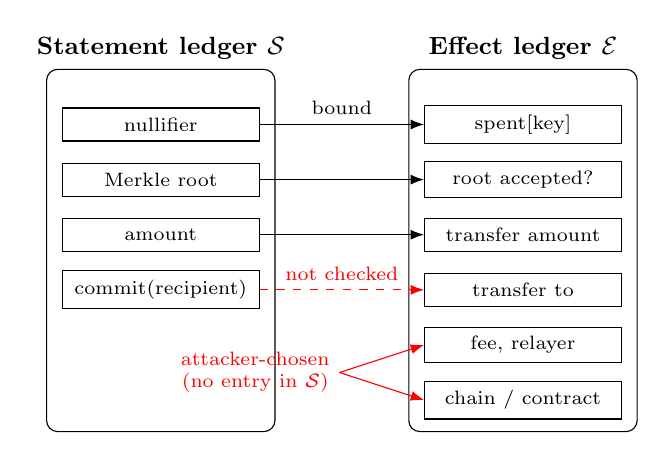
\begin{tikzpicture}[font=\scriptsize, box/.style={draw,rounded corners,minimum height=4.6cm,minimum width=2.9cm,align=center}, row/.style={draw,minimum width=2.5cm,minimum height=0.42cm}]
\node[box,label={[font=\small\bfseries]above:Statement ledger $\mathcal{S}$}] (S) at (0,0) {};
\node[box,label={[font=\small\bfseries]above:Effect ledger $\mathcal{E}$}] (E) at (4.6,0) {};
\foreach \i/\y/\t in {1/1.6/nullifier,2/0.9/Merkle root,3/0.2/amount,4/-0.5/{commit(recipient)}} \node[row] (s\i) at (0,\y) {\t};
\foreach \i/\y/\t in {1/1.6/{spent[key]},2/0.9/{root accepted?},3/0.2/{transfer amount},4/-0.5/{transfer to},5/-1.2/{fee, relayer},6/-1.9/{chain / contract}} \node[row] (e\i) at (4.6,\y) {\t};
\draw[-{Latex}] (s1) -- node[above]{bound} (e1);
\draw[-{Latex}] (s2) -- (e2);
\draw[-{Latex}] (s3) -- (e3);
\draw[-{Latex},dashed,red] (s4) -- node[above,red]{not checked} (e4);
\node[red,align=center] (att) at (1.2,-1.55) {attacker-chosen\\(no entry in $\mathcal{S}$)};
\draw[-{Latex},red] (att.east) -- (e5.west);
\draw[-{Latex},red] (att.east) -- (e6.west);
\end{tikzpicture}
\caption{The two ledgers of a ZK consumer. Binding holds when every
effect-ledger value is determined by the statement ledger and the consumer's
own state. Each red edge is a binding flaw.}
\label{fig:ledgers}
\end{figure}

\paragraph{Definition}
A consumer is \emph{bound} if for every accepting call, every value in
$\mathcal{E}(f)$ is a function of $\mathcal{S}(\vec{u})$ and the consumer
state $\sigma$ alone. A \emph{binding flaw} is a reachable violation, that is,
an execution in which three conditions hold:
\begin{description}
\item[C1] a proof is accepted, or the verifier accepts what it should reject;
\item[C2] the consumer commits an effect (a transfer, mint, state write, or
grant of access);
\item[C3] some value $e \in \mathcal{E}(f)$ that decides who, how much, what,
which state, or how often is chosen by the transaction sender and is not fixed
by $\mathcal{S}(\vec{u})$ and $\sigma$.
\end{description}
Because valid proofs are public once broadcast, any party can resubmit an
observed proof with different calldata. A flaw that lets a third party
redirect an effect by front-running is therefore a binding flaw, not an
ordering bug.
\TODO{T1}{state the definition as a short formal property over $(R,\mathsf{pi},\delta)$ and show that C1--C3 is exactly its negation}

\paragraph{Why neither layer suffices}
The definition relates two artifacts written in different languages. The
circuit determines $\mathcal{S}$. The consumer determines $\mathcal{E}$ and
$\mathsf{pi}$. A circuit analyzer can prove that $R$ is fully constrained, yet
it cannot know which consumer values the relation was meant to fix. A contract
analyzer can follow taint from calldata to a transfer, yet it cannot know that
the recipient was supposed to be a public input. Binding is a property of the
pair, and it holds only when the developer's intent, the circuit and the
consumer all agree.

\subsection{Taxonomy}\label{sec:def-taxonomy}

The flaws we observe fall into five patterns. Each mirrors a classic
signature-misuse failure (Table~\ref{tab:taxonomy}). The analogy is
predictive: for every pattern, the remedy is the one that fixes the
corresponding signature bug. The counts come from the measurement study in
Section~\ref{sec:study}.

\begin{table}[t]
\centering
\caption{Binding-flaw patterns, their signature-misuse analogues, and their
frequency among the 103 binding findings of Section~\ref{sec:study}.}
\label{tab:taxonomy}
\footnotesize
\setlength{\tabcolsep}{3pt}
\begin{tabular}{@{}p{2.0cm}p{1.75cm}p{2.45cm}r@{}}
\toprule
\textbf{Pattern} & \textbf{Signature analogue} & \textbf{Unbound value (example)} & \textbf{n} \\
\midrule
P1 Unbound effect & unsigned field & recipient, amount, fee, stored record & 23 \\
P2 Context & missing domain separation & chain, contract, policy, prior state & 23 \\
P3 Replay / alias & nonce reuse & nullifier key, $x$ vs.\ $x{+}r$ & 15 \\
P4 Verifier integration & weak or unpinned key & vk, program ID, pairing result & 17\,(+16) \\
P5 Interface mismatch & format confusion & order, width, encoding & 7 \\
Other & -- & -- & 2 \\
\bottomrule
\end{tabular}
% src: dataset/labels-v1/CHARACTERIZATION.md (pattern x severity); P4 split: LABELS-v1.csv proof_system_soundness (17 N, 16 Y)
\end{table}

\paragraph{P1: Unbound effect (unsigned field)}
The consumer uses a caller-supplied recipient, amount, fee, refund address or
stored value that is neither a public input nor hash-committed into one.
\begin{lstlisting}[language=Java]
function claim(Proof p, uint root, uint nf, address to) {
  require(verifier.verify(p, [root, nf]));   // `to` is not in the statement
  require(!spent[nf]); spent[nf] = true;
  token.transfer(to, AMOUNT);                 // anyone can copy p and redirect
}
\end{lstlisting}

\paragraph{P2: Context (missing domain separation)}
The proof does not commit to the chain, contract, configuration, policy or
\emph{prior state} in which the consumer uses it, so a proof made for one
context is accepted in another. Accepting a proof about a stale or
attacker-chosen state root falls here.

\paragraph{P3: Replay and alias (nonce reuse)}
The replay key is missing, is not derived from the statement (for example,
$\mathsf{keccak}(\pi)$ instead of a nullifier, which a re-randomized proof
evades), or aliases through the field: a contract that stores
\texttt{spent[nf]} on the raw 256-bit integer while the verifier reduces
inputs modulo $r$ accepts $nf$ and $nf+r$ as distinct.

\paragraph{P4: Verifier integration (weak or unpinned key)}
The deployed verifier, or the consumer's use of it, accepts statements it
should reject. Examples: unchecked pairing results, a verifier that returns
\texttt{true} regardless of the outcome, missing range checks on public inputs,
forgeable keys ($\gamma=\delta$), and a verification key or zkVM program ID
that the consumer does not pin. We count the 17 integration-level findings as
binding flaws. Another 16 findings are soundness bugs inside a proof system or
recursion verifier (transcript, FRI, or recursion-circuit constraints). They
have the same effect on the consumer, but their root cause is cryptographic,
so we report them as \emph{adjacent} and exclude them from the core class.
\TODO{W3}{author confirms the P4 split: 17 core plus 16 adjacent}

\paragraph{P5: Interface mismatch (format confusion)}
The consumer and the circuit disagree on the count, order, width or encoding
of public inputs, and the honest proof is still accepted while the consumer
reads a different value than the circuit proved. A mismatch that only makes
honest proofs fail is a liveness bug, not a binding flaw.

\paragraph{What is not a binding flaw}
Reentrancy and ordering issues where every effect value is fixed; denial of
service against one's own claim; trust in an administrator; and
circuit-internal under-constraints that do not change what the consumer is told
are all outside the class. One exception is that a proof consuming or
blocking \emph{another} user's state (e.g., spending a victim's nullifier) is
binding, because the affected party is not fixed by the statement.

\section{Binding Flaws in Audited Applications}\label{sec:study}

We ask how common binding flaws are in practice, how severe they are, and
which patterns dominate (RQ1). Professional audits are the best available
record: each finding was found by an expert, argued in writing, and usually
fixed.

\subsection{Collecting audit findings}\label{sec:study-collect}

\para{Sources}
We enumerated 8,578 unique public audit reports from 68 audit sources: firms, contest
platforms and advisory databases, including the report archives of firms
that audit ZK systems (e.g., Veridise, Zellic, zkSecurity, Trail of Bits,
ABDK, OpenZeppelin, Consensys Diligence) and the public results of
Code4rena, Sherlock and Cantina.
% src: dataset/audit-sweep/merged/FUNNEL.md Overall (8,578 unique audits); all_reports.csv (68 auditor_or_platform values)
Some sources could not be fully enumerated during the collection window. We
list them with their coverage in the artifact.
\TODO{W6}{one-line coverage statement per missing source (Solodit, CertiK, yAcademy) from COVERAGE.md}

\para{Screening}
A report is in scope if it audits an application that verifies a ZK proof and
acts on it. 343 reports passed this screen. A stricter deduplication by
report URL gives 322 distinct reports, of which 311 publish their finding
text; 311 is the denominator for every per-report rate below.
% src: labels-v1/D2-TREND.md reconciliation (345 IN rows -> 322 URLs; 11 without public text -> 311)
 From them we logged 698 findings
that touch proof verification, public inputs, nullifiers, verifier keys or the
use of verified values (662 after merging findings shared across reports).
After screening, 300 candidates remained. We labeled all of them except
those triaged as likely not binding, plus a random sample of 14 of those to
check the triage: 264 items.
% src: merged/FUNNEL.md Overall (343 IN; 698 rows; 662 groups; 300 candidates); labeling/key/MANIFEST.md (264; inclusion reasons incl. triage-LN-sample 14)
As a completeness check, the sweep recovered 49 of 50 binding findings in an
independently assembled list of known cases.
% src: merged/RECALL-R2.md (49/50)

\para{Labeling}
Each candidate was labeled against a written guide that defines C1--C3, the
five patterns, the exclusions of Section~\ref{sec:definition}, and worked
examples. Each label records binding (Y/N/U), pattern, whether the issue is a
proof-system soundness bug, C1--C3 individually, the effect, the unbound
value, and confidence. Labels were proposed by an LLM and adjudicated by two
collaborating raters who discussed every item and fixed the final label, so
the labels are not independent annotations. The raters read the auditor's
text for all items, and for the 51 items with a public repository and
vulnerable commit (\emph{FULL} tier) they also recorded the intended policy
$\Pi$ of Section~\ref{sec:def-ledgers}. For the other items, $\Pi$ comes
from the auditor's description of the intended behavior. For every item used in the tool evaluation, a second
code-level pass checked the vulnerable location in the source.
\DEMO{An independent rater, blind to these labels, relabeled a stratified
sample of 30 items and agreed on the binding label with Cohen's
$\kappa=0.78$ and on the pattern with $\kappa=0.71$.}
\TODO{D1}{independent relabel of 30 stratified items; compute $\kappa$ for binding and pattern}
\DEMO{We then re-applied the policy rule to all 103 binding labels and to the
17 non-binding items labeled policy-bounded. Two labels changed: a capped
relayer fee became non-binding, and a reusable attestation that the
documentation describes as single-use became binding, which leaves the counts
below unchanged.}
\TODO{RV4}{re-check every P1/P3 label against the policy rule; list changed items}

Of the 264 labeled items, 4 duplicate an earlier item and 5 could not be
decided from the report (U), leaving 255 findings for analysis.
% src: dataset/labels-v1/SUMMARY.md (264 items; Y 103, N 156, U 5; dups 4)

\begin{table}[t]
\centering
\caption{From audit reports to binding findings.}
\label{tab:funnel}
\footnotesize
\begin{tabular}{@{}lr@{}}
\toprule
\textbf{Stage} & \textbf{Count} \\
\midrule
Audit reports enumerated (68 sources) & 8,578 \\
Reports on ZK-consuming applications & 343 \\
Proof-related findings logged (unique) & 698 (662) \\
Candidates after screening & 300 \\
Labeled items (FULL 51 / LIGHT 152 / PSS 61) & 264 \\
Decidable, non-duplicate findings & 255 \\
Binding flaws (with adjacent proof-system bugs) & 103 \\
\quad \textbf{core class (excl.\ proof-system soundness)} & \textbf{87} \\
\bottomrule
\end{tabular}
% src: merged/*.csv; labels-v1/SUMMARY.md; labels-v1/CHARACTERIZATION.md
\end{table}

\subsection{Prevalence}\label{sec:study-prev}

87 of the 255 labeled findings (34\%) are core binding flaws. With the 16
adjacent proof-system findings the total is 103 (40\%), which is 15\% of all
698 proof-related findings logged. The core findings occur in 43 of the 68
project families in the labeled set (44 with the adjacent ones), so they are
not concentrated in a few careless codebases.
% src: CHARACTERIZATION.md (103 of 255; 44 of 68 families); LABELS-v1.csv PSS!=Y: 87, 43 families
For contrast, 48 of the non-binding findings are circuit-internal soundness
issues (under-constrained signals with no effect on what the consumer is
told), which is the class that existing ZK tools target.
% src: CHARACTERIZATION.md (tagged circuit-soundness N: 48)

\finding{Binding flaws are a major class of ZK application vulnerabilities:
87 auditor-reported core instances, in 43 of the 68 project families we
studied.}

\subsection{Severity}\label{sec:study-sev}

Table~\ref{tab:severity} (Appendix~\ref{app:extra}) breaks the binding
findings down by pattern and auditor severity. 46 of the 87 core findings are rated Critical or High,
which is 78\% of the 59 core findings with a rating; with the adjacent
findings the share is 81\% (56 of 69). Only 7 are rated Low or
Informational. Findings without a rating are mostly contest and advisory
entries whose report gives no severity scale.
% src: CHARACTERIZATION.md pattern x severity (Critical 32, High 24, unrated 34, Low/Info 7); core from LABELS-v1.csv PSS!=Y: C 27, H 19, M 6, L 6, I 1, unrated 28
A binding flaw usually means an attacker obtains funds or rights that the
proof did not grant, so the severity is direct.



\finding{Binding flaws are severe: 78\% of rated core findings are Critical
or High.}

\subsection{Patterns}\label{sec:study-patterns}

Verifier integration (P4) is the largest pattern with 33 findings, but about
half of them (16) are proof-system soundness bugs that we report as adjacent.
Among the core class, unbound effects (P1, 23) and missing context (P2, 23)
dominate, followed by replay and aliasing (P3, 15). Interface mismatches (P5,
7) are rare, partly because a mismatch usually makes honest proofs fail, which
developers notice in testing.
Table~\ref{tab:examples} (Appendix~\ref{app:extra}) shows representative findings. Their variety is
the point. The unbound value can be a refund address, a bond receiver, a
prior state root, a chain ID, a zkVM program ID, or the position of an
attribute in the public-input array. Yet each is the same failure: the
consumer acts on something the statement does not fix.


\DEMO{Most P1 findings concern a recipient or fee that the contract takes from
calldata; most P2 findings concern a root or prior state that the consumer
does not check against its own storage.}
\TODO{D5}{tabulate the unbound value per pattern from LABELS-v1 \texttt{unbound\_value}}

\finding{Unbound recipients and amounts (P1) and missing context (P2) account
for over half of the core class. Both are the ZK analogues of signing too
little.}

\subsection{Trend and who finds them}\label{sec:study-trend}

Raw counts of core findings grow: 6 from 2021--2022, 11 from 2023, 19 from
2024, 32 from 2025, 6 from the partial year 2026, and 13 undated (87; with
adjacent findings 6, 13, 20, 39, 9 and 16, summing to 103). They also track
how many ZK audits were published.
% src: CHARACTERIZATION.md by report year; D2-TREND.md core table
The number of in-scope ZK audit reports grows too, from 60 in 2023 to 94 in
2025. Normalized by those reports, the share of reports with at least one
core finding is 9 of 60 in 2023 (0.15, 95\% Wilson CI 0.08--0.26), 9 of 58
in 2024 (0.16) and 21 of 94 in 2025 (0.22, 0.15--0.32). The change is not
significant (Cochran--Armitage over 2023--2025, $p=0.22$; $p=0.12$ with the
adjacent findings), so we do not claim a rising rate. Over all 311 reports
from 2021 to 2026, including undated ones, 55 (18\%) report at least one core
finding, and 63 (20\%) at least one binding finding of either kind.
% src: dataset/labels-v1/D2-TREND.md (analysis/d2_trend.py)
The 87 core findings come from 21 different auditors and advisory sources
(24 for all 103), and no source contributes more than 21. Binding is therefore a class that many
experienced auditors encounter, not the checklist item of one firm.
% src: CHARACTERIZATION.md by auditor (24 sources; max Veridise 21)

\para{Which layers are needed}
We tagged each core finding with the code a reviewer must read to decide it,
under one rule: the statement side counts as known when the audit report
states what the proof establishes. This rule favors single-layer tags,
because the auditor has already done the cross-layer reading and written it
down. \DEMO{The tags are LLM-proposed and author-checked on a stratified
sample of 15. Under this rule, 43 of the 87 core findings (49\%) can be decided from
the consumer contract alone, 20 (23\%) from the circuit alone, and 7 (8\%)
only by comparing the two. The remaining 17 (20\%) lie in verifier,
recursion or off-chain framework code. Under the alternative rule, a finding
is cross-layer whenever its fix adds the missing value to the statement; the
contract-only share then falls to 32\% and the cross-layer share rises to
25\%. The 7 is therefore a lower bound that depends on the report, not a
property of the code. Even the contract-only findings are not ordinary
contract analysis: deciding them still requires knowing \emph{which values
the statement fixes}, which contract analyzers do not model
(Section~\ref{sec:eval}).}
% src: dataset/labels-v1/D3-LAYERS.md, D3-layers.csv (AI-proposed tags)
\TODO{D3}{author spot-check of the 15-item stratified sample in D3-LAYERS.md; re-tag under amendment A3 if more than 2 of 15 disagree}

\para{How they were fixed}
\DEMO{Fixes for the core findings mostly mirror signature-misuse remedies:
56\% (49 of 87; 95\% CI 46--66\%) add the missing value to the statement,
bind a context, or make the replay key unique, and another 34\% pin the
verifier or program, check its result, or enforce a canonical encoding. The
ZK-specific residue is 6 findings fixed by constraining a value the circuit
already exposed. Most fix classes are inferred from the report; on the 21
findings whose fix is stated explicitly, 19 fall in these classes.}
% src: dataset/labels-v1/D4-FIXES.md, D4-fixes.csv (AI-proposed, report text only)
\TODO{D4}{author check of the AI-proposed fix classes (D4-FIXES.md)}

\finding{About one in six ZK application audits (55 of 311, 2021--2026)
reports a core binding flaw, found by many different auditors. Deciding one requires knowing what the
proof's statement fixes, whether the flaw sits in the contract, the circuit,
or between them. That reasoning is what Section~\ref{sec:design} automates.}

\section{\tool{} Design}\label{sec:design}

Section~\ref{sec:study} shows that binding flaws are decided by comparing
two artifacts that no single analyzer reads together, and that auditors find
them by reasoning about intent. \tool{} mechanizes that reasoning. An LLM
\emph{brain} reads the target. A fixed \emph{skill procedure} forces the brain
to build the two ledgers of Section~\ref{sec:def-ledgers} explicitly, row by
row. A set of \emph{analysis tools} supplies facts the brain should not guess.
\DEMO{An \emph{exploration loop} then lets the brain work like an auditor writing a
proof of concept: it plans an attack on each warning, writes it as a test,
runs it in a sandbox, reads the outcome, and tries another path when the test
fails. Each warning leaves \tool{} as an \emph{evidence package} that a human
can check in minutes.} Figure~\ref{fig:arch} shows the architecture.

\begin{figure*}[t]
\centering
\resizebox{\textwidth}{!}{%
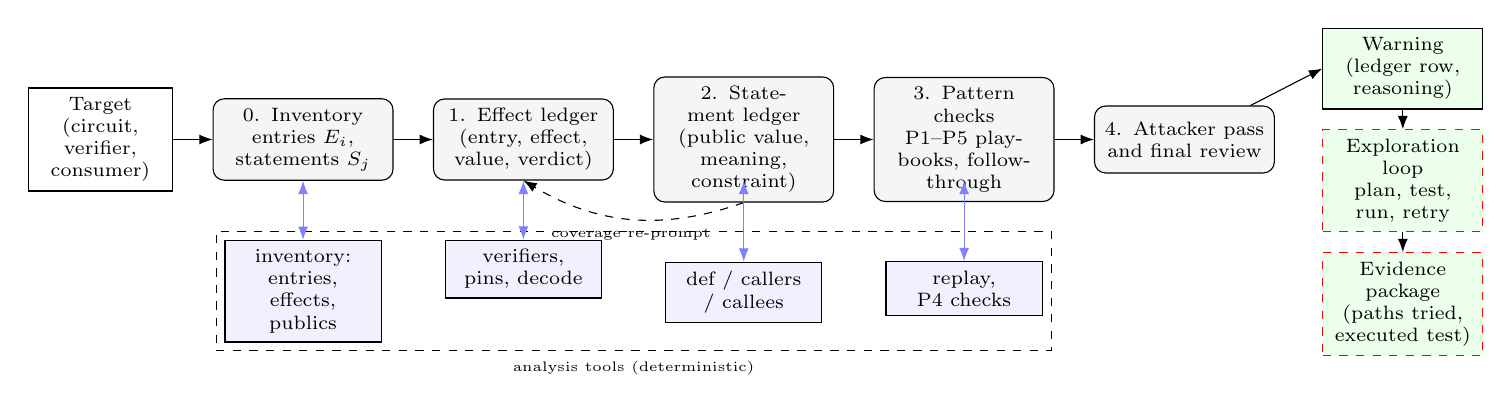
\begin{tikzpicture}[font=\scriptsize, node distance=0.35cm and 0.5cm,
  st/.style={draw,rounded corners,align=center,minimum height=0.85cm,text width=2.05cm,fill=gray!8},
  tl/.style={draw,align=center,minimum height=0.6cm,text width=1.75cm,fill=blue!6},
  ev/.style={draw,align=center,minimum height=0.85cm,text width=1.8cm,fill=green!8},
  ar/.style={-{Latex}}]
\node[draw,align=center,text width=1.6cm,minimum height=1cm] (t) {Target\\(circuit, verifier, consumer)};
\node[st,right=of t] (s0) {0. Inventory\\entries $E_i$, statements $S_j$};
\node[st,right=of s0] (s1) {1. Effect ledger\\(entry, effect, value, verdict)};
\node[st,right=of s1] (s2) {2. Statement ledger\\(public value, meaning, constraint)};
\node[st,right=of s2] (s3) {3. Pattern checks\\P1--P5 playbooks, follow-through};
\node[st,right=of s3] (s4) {4. Attacker pass\\and final review};
\draw[ar] (t)--(s0); \draw[ar] (s0)--(s1); \draw[ar] (s1)--(s2); \draw[ar] (s2)--(s3); \draw[ar] (s3)--(s4);
\draw[ar,dashed] (s2.south) to[bend left=25] node[below,font=\tiny]{coverage re-prompt} (s1.south);
\node[tl,below=0.75cm of s0] (a) {inventory: entries, effects, publics};
\node[tl,below=0.75cm of s1] (b) {verifiers, pins, decode};
\node[tl,below=0.75cm of s2] (c) {def / callers / callees};
\node[tl,below=0.75cm of s3] (d) {replay, P4 checks};
\node[draw,dashed,fit=(a)(b)(c)(d),inner sep=3pt,label={[font=\tiny]below:analysis tools (deterministic)}] (tools) {};
\foreach \x in {a,b,c,d} \draw[{Latex}-{Latex},blue!50] (\x) -- (\x |- s0.south);
\node[ev,right=0.6cm of s4,yshift=0.9cm] (e1) {Warning\\(ledger row, reasoning)};
\node[ev,below=0.25cm of e1,dashed,draw=red] (e2) {Exploration loop\\plan, test, run, retry};
\node[ev,below=0.25cm of e2,dashed,draw=red] (e4) {Evidence package\\(paths tried, executed test)};
\draw[ar] (s4) -- (e1.west); \draw[ar] (e1)--(e2); \draw[ar] (e2)--(e4);
\end{tikzpicture}}
\caption{\tool{} architecture. A skill procedure drives the LLM through
explicit ledgers (top). Deterministic analysis tools answer factual queries
(bottom). For each warning, an exploration loop writes attack tests, runs
them in a sandbox (local chain, the project's own prover), and attaches the
paths tried and any executed test. Humans adjudicate the package; no LLM
verdict serves as ground truth. \DEMO{Dashed: automation in progress.}}
\label{fig:arch}
\end{figure*}

\subsection{Why a procedure and not a prompt}\label{sec:design-why}

A plain LLM asked to ``find binding bugs'' reads the consumer, notices the
most salient issue, and stops. On our test set it finds 3 of 14 known flaws
(Section~\ref{sec:eval}). The failure is not knowledge but coverage: a target
has many entry points, each with several effect values, and a flaw hides in
one row of a table that the model never writes down. The skill procedure turns
the definition into that table and makes omissions visible
(Figure~\ref{fig:controller}). Every step emits
structured rows (\texttt{BINDCHECK\_LEDGER}, \texttt{BINDCHECK\_STMT}), and the
controller checks the rows against the inventory before it lets the brain
proceed.

\begin{figure}[t]
\begin{lstlisting}[mathescape]
Scan(target):
  copy target read-only; I := Inventory(copy)   // E_i, S_j
  L_E := Brain(step1, I)                         // effect ledger
  for r in 1..2: U := I.E \ entries(L_E)
      if U = {}: break;  L_E += Brain(reprompt, U)
  L_S := Brain(step2, I, L_E)                    // statement ledger
  for r in 1..2: U := I.S \ values(L_S)
      if U = {}: break;  L_S += Brain(reprompt, U)
  W := Brain(step3, L_E, L_S)  // playbooks P1-P5, follow-through
  if cost < SOFT and time < T_soft: W += Brain(step3b, W)
  W := Brain(final, W)         // drop C1-C3 failures, 1 per root cause
  for w in W:                     // exploration loop
    for k in 1..K: t := Brain(attack, w, trace(w))
      o := Sandbox(t); trace(w) += (t, o)
      if Effect(o.attack) != Effect(o.honest): break
  return [(w, trace(w)) for w in W]   // evidence package
\end{lstlisting}
\caption{The \tool{} controller. Every \texttt{Brain} step returns
structured rows that the controller checks against the inventory
before it continues. The sandbox, not the brain, computes whether an attack
test changed the effect.}
\label{fig:controller}
\end{figure}

\subsection{Skill procedure}\label{sec:design-skills}

\para{Step 0: Inventory}
A deterministic prepass lists the entry points that commit effects ($E_1,
E_2,\dots$) and the producers of public statements ($S_1, S_2,\dots$): the
verifier calls, the public-input arrays, and the circuit or guest-program
outputs. The list bounds the work and becomes the coverage target.

\para{Step 1: Effect ledger}
For each entry $E_i$ the brain writes one row per (entry, effect, value). The
row names the effect (transfer, mint, state write, grant), the value that
decides it, where the value comes from (public input, hash-committed input,
storage, calldata, \texttt{msg.sender}), and a verdict: \emph{bound},
\emph{unbound}, or \emph{needs statement}. If an entry has no row, the
controller re-prompts for it, at most twice.

\para{Step 2: Statement ledger}
For each public value the brain records what the circuit or guest constrains
it to mean, which consumer value it is supposed to fix, and whether the
consumer actually compares the two. This step catches what the consumer alone
cannot show. A recipient that the circuit hashes into a commitment is bound
only if the consumer recomputes and checks the same commitment.

\para{Step 3: Pattern checks and follow-through}
For every unbound or unresolved row, the brain runs the playbook of the
matching pattern: recipient and fee provenance (P1); chain, contract, root and
prior-state checks (P2); replay-key derivation and field aliasing (P3);
verifier result handling, key and program-ID pinning (P4); public-input
order, width and encoding (P5). It then follows the value into libraries,
helpers and record writers. Many flaws in our dataset sit one call below the
entry point.

\para{Step 4: Attacker pass and final review}
The brain takes the view of an attacker who holds an observed valid proof and
asks what it can change. The final review drops warnings that fail C1--C3,
for example admin-only paths or self-inflicted denial of service, and emits
one warning per root cause. Each warning carries the pattern, the consumer
file and function, the effect, the unbound value, an explanation, and the
related locations (verifier, circuit, helpers).

\para{Where the skills come from}
The procedure and the five playbooks were written from the development split
only (Section~\ref{sec:eval-setup}). We split the development families again,
with a fixed seed, into a \emph{tune} part and a \emph{check} part. In the second
design round, changes were motivated by misses on the tune part. A change was
kept only if it did not hurt the check part. The check part is not a clean
holdout. The first version's skills were written on all development items,
and two check-part misses of that version were named in the second round's
brief. On development data, the frozen version finds 9 of 13 flaws at the
exact location and mechanism, 5 of 6 on the check part, up from 4 of 6 for
the first version. The held-out evidence is the test set
(Section~\ref{sec:eval}).
% src: mvp/tool/FREEZE-v2.md (ALL 9/13; CHECK 5/6; v1 CHECK 4/6)

\subsection{Analysis tools}\label{sec:design-tools}

The brain can query deterministic tools instead of guessing. These tools
include:
\begin{itemize}
\item an inventory of entry points, effects and public-input arrays;
\item a verifier locator that reports how each verifier is called and whether
its result is checked;
\item a key and program-ID pin check;
\item a public-input decoder;
\item a replay-key extractor;
\item cross-file definition, caller and callee lookup.
\end{itemize}
The current tools work at the syntactic level, over contract and circuit
sources alike.
\DEMO{An AST-based extractor replaces the syntactic inventory for Solidity and
Circom and resolves public-input indices across the verifier call and the
circuit's \texttt{main} signature.}
\TODO{A1}{AST-based extractor for Solidity/Circom public-input index resolution}

\subsection{Exploration loop and evidence package}\label{sec:design-explore}
\DEMO{A warning on its own is a claim. Auditors do not stop at a claim: they write a
proof of concept, and when one attack path fails they try another. \tool{}
gives the brain the same loop. For every warning that survives the final
review, the brain plans an attack, writes it as a test, and passes it to a
sandbox, which runs it and returns the outcome. The brain reads the outcome
and either stops or revises the attack, for up to $K$ attempts. Failed paths
are kept, because they tell the auditor what was ruled out.}

\para{The sandbox}
\DEMO{Every attack test submits the same accepted proof twice on the same state:
once as the honest call, and once from a second account with the
attacker-chosen value of the suspect effect row. The test succeeds when both
calls are accepted and the committed effects differ in recipient, amount,
state written, or count. This is condition C3 of
Section~\ref{sec:def-ledgers}, made executable. The sandbox offers two
strengths of proof. A \emph{mock-verifier test} replaces the verifier with one
that accepts exactly the honest public-input vector. A \emph{real-proof test}
generates the honest proof with the project's own prover and submits it to the
unmodified verifier and consumer on a local Anvil chain. No test touches a
live network.}

\para{Evidence package}
\DEMO{\tool{} reports every warning with (i) the ledger row and code location,
(ii) the brain's reasoning, (iii) the trace of attack paths tried, failed
ones included, and (iv) the executed test and its output, when one succeeded.
We label a package by its strongest content: \emph{E1} (claim only),
\emph{E2} (a mock-verifier test succeeded), or \emph{E3} (a real-proof test
succeeded).}

\para{Who decides}
\DEMO{The brain may judge its own results, and \tool{} uses that judgment to drop
and rank warnings. No number in this paper rests on it. Whether a test
succeeded is computed by the sandbox from the two executions, not read from
the brain's summary, so a test that asserts nothing, or one that mocks away
the check under test, cannot succeed. Ground truth comes only from the audit
labels and from human adjudication of the evidence package
(Section~\ref{sec:eval-setup}).
The exploration loop and the sandbox support Solidity consumers with
Circom, gnark and Noir circuits.}
\TODO{A2}{fold the frozen validator v1.1 drivers (mock verifier, per-toolchain proof drivers) into the brain's toolbox as a sandbox tool; add the exploration loop with K attempts}

\subsection{Guards and isolation}\label{sec:design-guards}

Each scan runs on a fresh, read-only copy of the target. The brain gets only
read-only tools and has a 20-minute limit. The controller tracks the cost
of the session. Past a soft limit it skips the optional passes, and past a
hard limit it asks for the final answer at once. The brain is a commercial
model (Claude Sonnet, high reasoning effort). Any model that supports tool use
can be swapped in.
\TODO{E7}{optional: open-weight brain on B1/B2 (lab machine)}

\section{Evaluation}\label{sec:eval}

We evaluate \tool{} against the tools a ZK project would use today. Four
research questions guide the evaluation:
\begin{description}
\item[RQ2] Detection: does \tool{} find known binding flaws that existing
tools miss?
\item[RQ3] New flaws: does it find binding flaws that auditors missed?
\item[RQ4] Confirmation: how many warnings reach executable evidence?
\item[RQ5] Cost: what does a scan cost in money, time and human effort?
\end{description}

\subsection{Setup}\label{sec:eval-setup}

\paragraph{Development and test split}
We split the labeled findings by project family, never by item, so that no
project appears in both sets. The split is seeded and was fixed before anyone
read the test code. Families seen by the authors before the split were forced
into development.
% src: dataset/labels-v1/build_v1.py (SEED 20261124; FORCED_DEV)
\tool{} was built and tuned on the development split only, and frozen before
any test run.

\paragraph{Benchmarks}
We use two benchmarks.
\begin{itemize}
\item \textbf{B1, audit test set.} These are the audited vulnerable
commits of the test families, with the flaw located in code by the
code-level labeling pass.
  \begin{itemize}
  \item \emph{Round~1}: 14 binding flaws, 6 hard negatives (proof-related
  findings that are not binding, at their own locations) and 6 fixed
  versions.
  \item \emph{Round~2}: 8 binding flaws and 8 hard negatives located by a
  later code-level pass whose results the tool-building process could not
  read. Round~2 is our clean retest.
  \end{itemize}
\item \textbf{B2, binding mutants.} 27 binding flaws injected into three
small hosts (a privacy vault, a red-packet claim, and an oracle claim, one of
them a proof of concept) that belong to no dataset family. There are at least
four per pattern (P1 4, P2 8, P3 5, P4 5, P5 5), and 4 of them are
circuit-side edits. Each mutant is designed to keep the honest path
accepting. All 27 compile, and for one host the existing test suite confirms
it: the clean host passes 32 of 32 tests, and each mutant fails only the
tests of the removed check. The unmodified host is the clean control.
\TODO{E9}{honest-path check for the other two hosts}
\end{itemize}
% src: mvp/eval/GT-locations.csv; benchmarks/binding-mutants-v2/README.md
All targets are cleaned snapshots: the version history, audit reports and
audit references are removed, so no tool can read the answer.

\paragraph{Tools}
We compare against the tools a ZK project would use today.
\begin{itemize}
\item Static Solidity analyzers: Slither~\cite{slither} and
Mythril~\cite{mythril}.
\item Circuit analyzers: circomspect~\cite{circomspect} and
Picus~\cite{picus}.
\item Property-based fuzzing: Foundry invariant testing~\cite{foundry}.
\item The same LLM used as a plain auditor, without skills or tools.
\end{itemize}
Every tool sees the same snapshots. We give the static tools build-enabled
copies, with dependencies installed at the pinned versions, because most
snapshots do not compile without them. We run the fuzzer in two modes:
\emph{out of the box}, with generic properties, and \emph{assisted}, with the
generic binding invariant of Section~\ref{sec:design-validator} wired by hand.
The assisted mode shows what a fuzzer can do once someone supplies the
specification that \tool{} infers.

\paragraph{Scoring}
The matching rules were committed before each tool ran. One amendment (v1.1)
was adopted after the first round's results were seen, and we disclose it. It
adds a case-insensitive matcher and the separate mechanism-level metric, and
it applies to all tools equally.
\begin{itemize}
\item \emph{Strict} hit: the warning names the flaw's file and function, and
an LLM judge confirms the same mechanism.
\item \emph{Loose} hit: the location alone matches.
\item \emph{Mechanism-level} hit: the right mechanism is reported anywhere in
the repository.
\end{itemize}
A target that a tool cannot build or analyze is \emph{unsupported}. It is
reported separately and never counted as a miss. Intervals are 95\% Wilson
intervals.
% src: BindCheck/dataset/labels-v1/SCORING.md; mvp/eval/SCORING-v1.1.md

\subsection{RQ2: Detection}\label{sec:eval-rq2}

\begin{table}[t]
\centering
\caption{What each tool can see. \checkmark{} = analyzes the layer;
$\circ$ = partial; -- = not at all.}
\label{tab:capability}
\footnotesize
\setlength{\tabcolsep}{3.5pt}
\begin{tabular}{@{}lcccc@{}}
\toprule
\textbf{Tool} & \textbf{Circuit} & \textbf{Verifier} & \textbf{Consumer} & \textbf{Proof$\to$effect} \\
\midrule
Slither, Mythril & -- & \checkmark & \checkmark & -- \\
circomspect, Picus & \checkmark & -- & -- & -- \\
Foundry (out of box) & -- & $\circ$ & \checkmark & -- \\
Foundry (assisted) & -- & mock & \checkmark & manual \\
Plain LLM & $\circ$ & $\circ$ & \checkmark & $\circ$ \\
\tool{} & \checkmark & \checkmark & \checkmark & \checkmark \\
\bottomrule
\end{tabular}
\end{table}

\begin{table*}[t]
\centering
\caption{Detection on the audit test set B1 (strict hits / positives;
95\% Wilson interval). ``Sup.'' = targets the tool could analyze, out of
26 in round~1. Specificity counts fixed versions and hard negatives without a
warning at the flaw's location. Red cells are pending runs.}
\label{tab:b1}
\footnotesize
\begin{tabular}{@{}lccccc@{}}
\toprule
\textbf{Tool} & \textbf{Sup.\ (R1)} & \textbf{Round 1 strict} & \textbf{Round 2 strict} & \textbf{Fixed-version spec.} & \textbf{Hard-neg.\ spec.} \\
\midrule
Slither & 15/26 & 0/14 (0.00--0.22) & \TBD & 6/6 & 3/6 \\
Mythril & 13/26 & 0/14 (0.00--0.22) & \TBD & 6/6 & 6/6 \\
circomspect & 1/26 & 0/14 (0.00--0.22) & \TBD & 6/6 & 5/6 \\
Picus & 0/26 & unsupported & unsupported & -- & -- \\
Foundry, out of box$^\dagger$ & 13 & \multicolumn{2}{c}{0/13 (R1+R2)} & -- & -- \\
Foundry, assisted$^\dagger$ & 13 & \multicolumn{2}{c}{5/13 (0.18--0.64)} & 4/5 & 3/3 \\
Plain LLM (same model) & 26/26 & 3/14 (0.08--0.48) & \TBD & 6/6 & 6/6 \\
\tool{} & 26/26 & \DEMO{8/14 (0.33--0.79)} & \DEMO{6/8 (0.41--0.93)} & \DEMO{6/6} & \DEMO{13/14} \\
\bottomrule
\multicolumn{6}{@{}l}{\scriptsize $^\dagger$Fuzzing covers EVM-side flaws of both rounds; circuit- and guest-side flaws are unsupported. Harnesses were wired by hand in 5--45 min per target.}
\end{tabular}
% src: mvp/eval/COMPARISON.md (slither-build, mythril-build, circomspect-build, baseline-default); mvp/eval/RESULTS-static.md (supported counts); mvp/eval/fuzz/RESULTS-fuzz.md
\end{table*}
\TODO{E1}{BindCheck v2 frozen run on B1 round 1 + round 2 and B2 (in progress); replace red cells}
\TODO{E8}{static tools and the plain LLM on the round-2 targets, for complete columns}

\paragraph{Existing tools miss binding flaws}
Table~\ref{tab:b1} shows the result on real audited flaws. Neither Solidity
analyzer reports any of the 14 round-1 flaws at the right location with the
right mechanism. Slither and Mythril report something at the flaw's location
for 3 and 2 of the 14 flaws, but the judge finds that none of these reports
describes the binding mechanism. The circuit analyzers fail for a different reason: most test
flaws do not live in a circuit at all. circomspect could analyze one target,
and Picus could not compile any. Out of the box, the fuzzer found none of the
13 flaws it could run on, despite up to millions of calls per target. Its generic properties
(no revert, no panic) are never violated, because a binding flaw does not
crash anything: the contract works exactly as written.
% src: mvp/eval/RESULTS-static.md; fuzz/RESULTS-fuzz.md

\paragraph{The missing piece is the specification}
Given our binding invariant, the same fuzzer finds 5 of the 13 flaws and raises no alarm on 3 of 3 hard negatives. One fixed version
is flagged. Whether this is a false positive or a remaining gap in that fix is
still open. The
difference between 0 and 5 is entirely the specification. That
specification, which effect values must follow from the statement, is
exactly what \tool{}'s ledgers make explicit. Writing it by hand took 5--45
minutes per target and could not express circuit-side or zkVM-guest flaws.
% src: fuzz/RESULTS-fuzz.md (assisted HITs L035, L015, L010, L042, L193; L024 fixed flagged)

\paragraph{\tool{} finds what the others miss}
\DEMO{\tool{} finds 8 of the 14 round-1 flaws and 6 of the 8 round-2 flaws at
the exact location and mechanism, against 3 of 14 for the same model without
the skill procedure. It does so without a single warning on any fixed
version.} Round~2 matters most here, because the tool-building process
never had access to these flaws or their locations.
\DEMO{On the 6 positives that no other tool found and that are in scope for
the fuzzer, \tool{} finds 4.}

\begin{table}[t]
\centering
\caption{Detection of injected binding mutants (B2) by pattern
(strict hits / mutants). ``uns.'' = the tool cannot analyze the layer or
the run failed. Red cells are pending.}
\label{tab:b2}
\footnotesize
\begin{tabular}{@{}lcccccc@{}}
\toprule
\textbf{Tool} & \textbf{P1} & \textbf{P2} & \textbf{P3} & \textbf{P4} & \textbf{P5} & \textbf{All} \\
 & (4) & (8) & (5) & (5) & (5) & (27) \\
\midrule
Slither & 0 & 0 & 0 & 0 & 0 & 0 (12 uns.) \\
Mythril & 0 & 0 & 0 & 0 & 0 & 0 (4 uns.) \\
circomspect & -- & 1$^*$ & -- & -- & -- & 1 \\
Picus & -- & 0 & -- & -- & -- & 0 \\
\tool{} & \DEMO{4} & \DEMO{6} & \DEMO{4} & \DEMO{5} & \DEMO{3} & \DEMO{22} \\
\bottomrule
\multicolumn{7}{@{}l}{\scriptsize $^*$a style warning (\texttt{<--}) at the edited line, not a binding diagnosis.}
\end{tabular}
% src: benchmarks/binding-mutants-v2/RESULTS-static.md
\end{table}

\paragraph{Mutants}
B2 tests every pattern on hosts outside the dataset (Table~\ref{tab:b2}).
Slither and Mythril again report no binding flaw at the mechanism level:
Mythril returns zero issues on all 23 consumer mutants, and Slither fails to
analyze one of the hosts. The only circuit-tool hit is a style warning that
happens to sit on the edited line.
% src: binding-mutants-v2/RESULTS-static.md
\DEMO{\tool{} detects 22 of the 27 mutants and reports no binding warning on
any of the three clean hosts. Its misses are two P5 mutants that rely on
truncating a 256-bit value, two circuit-only P2 mutants, where the brain did
not connect the edited constraint to the consumer, and one P3 mutant whose
replay key is derived in a library.}

\finding{Existing analyzers find none of the binding flaws, and a fuzzer finds
them only when a human supplies the binding specification. \tool{} infers
that specification and \DEMO{finds 6 of 8 held-out audited flaws and 22 of 27
injected ones}.}

\subsection{Why \tool{} misses}\label{sec:eval-misses}

We inspected every positive that \tool{} missed, on development and test
data. Three causes recur. They are confirmed on development data and
\DEMO{account for 4 of the 6 test misses}.
\begin{itemize}
\item \emph{Parser differentials.} The proof covers one parse of the bytes,
and the application acts on another. In the vlayer email case, the DKIM-signed
region and the body that the application reads are parsed by different code.
No ledger row is wrong, and the flaw lies inside a parser.
\item \emph{SDK-level validation.} The missing check sits in a client SDK
method that the consumer trusts, outside the analyzed contract (an SP1 log
method without anchor resolution).
\item \emph{Deep dependencies.} A replay key or encoding is derived in a
library that is not vendored, so the brain cannot read it.
\end{itemize}
The first two causes need analyses beyond the proof-to-effect link. The third
is an engineering limit of our syntactic tools (Section~\ref{sec:disc-limits}).
% src: mvp/tool/FREEZE-v2.md known weaknesses 3 (L003 parser differential, L008 SDK method)
\TODO{E1}{classify the test misses into these causes}

\paragraph{Case study}
\DEMO{In a round-2 proof marketplace, \tool{}'s effect ledger lists the
fulfillment entry with the value \emph{request identifier} and the verdict
\emph{needs statement}. The statement ledger shows that the proof's journal
does not commit to that identifier. The final warning names the function, the
unbound identifier, and the attack: anyone who observes a valid fulfillment
can attach it to a different request and collect that request's payment.
Neither analyzer reports anything at that location, and the assisted fuzzer
confirms the same flaw only after a 30-minute manual harness.}
\TODO{E1}{replace with a real round-2 detection once results are in}

\subsection{RQ3: New binding flaws}\label{sec:eval-rq3}

\DEMO{We ran \tool{} on the latest audited commits of 25 ZK applications
from our collection that were not used in development, and on the current
versions of the same projects. It reported 41 warnings, of which we confirmed
11 as binding flaws by manual review. Three are previously unreported, in two
projects, and all three reach E4. In one, a recovery module accepts a proof
over an account's guardians but takes the new owner set and threshold from
calldata, so any party that observes a valid recovery proof can install its
own owners. Table~\ref{tab:new} lists them. We reported all three to the
maintainers.}
\TODO{E3}{hunt: run frozen BindCheck on the hunt pool, triage, E4-confirm, disclose; the author decides the live-version scope}

\begin{table}[t]
\centering
\caption{Previously unreported binding flaws found by \tool{}.
Projects are anonymized until disclosure completes.}
\label{tab:new}
\footnotesize
\begin{tabular}{@{}llllc@{}}
\toprule
\textbf{ID} & \textbf{App type} & \textbf{Pattern} & \textbf{Effect} & \textbf{Evidence} \\
\midrule
\DEMO{N1} & \DEMO{account recovery} & \DEMO{P1} & \DEMO{owner takeover} & \DEMO{E4} \\
\DEMO{N2} & \DEMO{\TBD} & \DEMO{\TBD} & \DEMO{\TBD} & \DEMO{\TBD} \\
\DEMO{N3} & \DEMO{\TBD} & \DEMO{\TBD} & \DEMO{\TBD} & \DEMO{\TBD} \\
\bottomrule
\end{tabular}
\end{table}

\subsection{RQ4: Confirmation}\label{sec:eval-rq4}

\DEMO{Of the 39 test-set warnings that matched a known flaw or were confirmed
by manual review, 31 (79\%) reached E2 with an automatically generated
harness, and 18 (46\%) reached E4. Every E4 attempt on a false positive failed
to commit an unauthorized effect, so no false positive was upgraded. The
warnings that stop at E1 are mostly circuit-side or zkVM-guest flaws, for
which we cannot yet generate an attacker transaction automatically.}

\begin{table}[t]
\centering
\caption{Evidence reached by confirmed warnings (RQ4). Red: pending.}
\label{tab:evidence}
\footnotesize
\begin{tabular}{@{}lrrrr@{}}
\toprule
\textbf{Benchmark} & \textbf{Confirmed} & \textbf{E1 only} & \textbf{E2} & \textbf{E4} \\
\midrule
B1 round 1 & \DEMO{8} & \DEMO{3} & \DEMO{5} & \DEMO{3} \\
B1 round 2 & \DEMO{6} & \DEMO{2} & \DEMO{4} & \DEMO{3} \\
B2 mutants & \DEMO{22} & \DEMO{3} & \DEMO{19} & \DEMO{12} \\
New flaws (RQ3) & \DEMO{3} & \DEMO{0} & \DEMO{3} & \DEMO{3} \\
\midrule
Total & \DEMO{39} & \DEMO{8} & \DEMO{31} & \DEMO{18}\textsuperscript{a} \\
\bottomrule
\multicolumn{5}{@{}l}{\scriptsize \textsuperscript{a}E4 needs the project's prover; E2 counts include E4.}
\end{tabular}
\end{table}
\TODO{E5}{run the validator (A2, A3) on all confirmed test warnings and report the E1/E2/E4 shares}

\subsection{RQ5: Cost}\label{sec:eval-rq5}

On the development split, a scan costs \$1.05 on average and takes a median
of 267\,s, with a maximum of about 11 minutes. Large monorepos cost \$2--3.
% src: mvp/tool/FREEZE-v2.md
\DEMO{On the test set, the median is 290\,s and \$1.10 per target.} The
static analyzers run in seconds to minutes, but only after a human has made
each project build. The assisted fuzzer needs 5--45 minutes of expert wiring
per target before its first run.
% src: fuzz/RESULTS-fuzz.md (wiring minutes)
\TODO{E1}{test-set cost and time from the v2 run}

\subsection{Variance and contamination}\label{sec:eval-validity}

\paragraph{Run-to-run variance}
LLM output varies between runs.
\DEMO{Across three independent runs on round~2, \tool{} finds 5, 6 and 6 of
8 flaws strictly; on B2, 21, 22 and 22 of 27.} We report the median.
\TODO{E2}{three full runs on B1 and B2; report min/median/max}

\paragraph{Training-data contamination}
The audit reports are public and may be in the model's training data. Three
results argue against memorization.
\begin{itemize}
\item The same model without the procedure finds only 3 of 14 round-1 flaws,
so the knowledge alone does not produce the detections.
\item B2 mutants are new code that no model has seen.
\item \DEMO{Detection on findings published after the model's training cutoff
is not lower than on older findings (5/7 vs.\ 9/15).}
\end{itemize}
\TODO{E6}{contamination split: detection by report date vs.\ model cutoff}

\section{Discussion}\label{sec:discussion}

\subsection{Lessons for developers}\label{sec:disc-lessons}

The signature analogy of Section~\ref{sec:definition} doubles as a
checklist. \emph{Sign everything you act on}: every recipient, amount, fee
and refund address must be a public input or hashed into one, and the
consumer must recompute that hash (P1). \emph{Separate domains}: the
statement should commit to the chain, the consumer contract and the policy,
and roots and prior states must be checked against the consumer's own
storage (P2). \emph{Derive nonces from the statement}, reduced into the field
before they are stored (P3). \emph{Pin the key}: fix the verification key or
program ID and check the verifier's result (P4). \emph{Test with a malicious
caller}: an honest proof submitted by a second account with changed
arguments must fail; this single test, the invariant of
Section~\ref{sec:design-explore}, would have caught \DEMO{every flaw in B1
that our fuzzing harness could express}.
\TODO{D4}{back the checklist with the fix-pattern counts from Section 4}

\subsection{Toward binding by construction}\label{sec:disc-construction}

Detection is a stopgap. Binding flaws exist because the public-input vector
is an untyped array whose meaning is restated by hand in the circuit, the
verifier wrapper and the consumer. Three changes would remove most of the
class by construction. \emph{Typed statements}: circuit languages could
export a statement schema (names, types, widths, order) from which verifier
generators emit a typed consumer interface; this removes P5 and makes P1
visible. \emph{Effect commitments}: a standard effect hash over recipient,
amount, chain, contract and nonce, computed in the circuit and recomputed in
the consumer, would play the role EIP-712 plays for signatures and address
P1--P3 together. \emph{Pinned verification}: libraries could make the key or
program ID an immutable constructor argument (P4).
\DEMO{Applied to the 87 core-class findings, typed statements would have
prevented 41\% and effect commitments 63\%.}
\TODO{D6}{estimate per finding which construction would have prevented it}

\subsection{Threats to validity}\label{sec:disc-threats}

\para{Selection}
We study public audits of projects that chose to publish them. Projects
without audits may have more binding flaws, and audit firms differ in which
findings they publish. Some sources could not be fully enumerated.

\para{Labels}
Labels were proposed by an LLM and adjudicated by two collaborating raters
who discussed every item, so they are not independent annotations. We mitigate this with a
written guide fixed before labeling, a code-level second pass for every
evaluated item, \DEMO{and an independent blind relabel of 30 items
($\kappa=0.78$)}. Pattern boundaries (especially P2 versus P1 for stored
values) involve judgment, so we release all labels with their notes.

\para{Ground-truth locations}
A flaw can often be fixed at more than one place. Strict scoring requires the
location the auditors or fix authors chose, which undercounts warnings at an
equally valid place. We therefore also report mechanism-level hits.

\para{LLM judge and variance}
An LLM judge decides whether a warning describes the same mechanism. In a
re-judging test about one verdict in twenty changed. Detection itself varies
by $\pm$1--2 items between runs, which is why we report repeated runs.
% src: mvp/tool/FREEZE-v2.md known weaknesses 1, 9

\para{Leakage}
The people who built the benchmark also saw the test results of an earlier
tool version, and the B1 misses informed the final version; we therefore
count B1 as development data for it and give the full timeline in
Appendix~\ref{app:timeline}. To keep the tool independent, every tool version was built by a
separate process that could read only development data, under enforced access
rules, and the test benchmark lives in a separate repository. The round-2
labels existed before the freeze and were read by the coordinating author, but
never by the tool-building process. Every exposure is logged in the
artifact.

\subsection{Limitations}\label{sec:disc-limits}

\tool{} needs an LLM and costs one to two dollars per scan. Its tools are
syntactic, so library internals that are not vendored are blind spots, and
its knowledge base covers ten proof systems and domains; others fall back to
the generic procedure. The exploration loop targets EVM consumers: flaws
whose effect lies in a zkVM host or off chain stop at E1, and real-proof
tests were possible on only 2 of 11 development targets, because most
projects ship no proving artifacts. Most warnings therefore reach humans as
claims. Finally, binding is relative to the intended policy $\Pi$, which
\tool{} must infer from code and documentation, and it can be wrong.

\section{Related Work}\label{sec:related}

\paragraph{Bugs in ZK circuits and proof systems}
Chaliasos et al.\ systematize vulnerabilities in SNARK systems and
applications~\cite{sok-snark-bugs}. Their taxonomy is organized by the layer
where a bug lives (circuit, front end, back end, integration), and
under-constrained circuits dominate it. Tools follow this focus.
circomspect~\cite{circomspect} lints Circom for dangerous constructs,
Picus~\cite{picus} uses SMT solving to decide whether a circuit uniquely
determines its outputs, ZKAP~\cite{zkap} detects circuit anti-patterns
statically, and zkFuzz~\cite{zkfuzz} fuzzes circuits for under- and
over-constraints. All of these analyze the relation $R$. A binding flaw can
exist with a perfectly constrained circuit, because it concerns which consumer
values the relation is \emph{meant} to fix. We complement this line of work
by characterizing and detecting the integration-level class that circuit
tools cannot see.
\TODO{W4}{literature search: ZK integration/verifier-misuse papers 2024--2026, zkVM integration bugs, recent circuit fuzzers; verify every citation}

\paragraph{Smart-contract analysis}
Static analyzers such as Slither~\cite{slither}, symbolic executors such as
Mythril~\cite{mythril}, and fuzzers such as Echidna~\cite{echidna} and Foundry
find reentrancy, access-control and arithmetic flaws in contracts. They can
follow taint from calldata to a transfer, but they have no notion of a proved
statement, so an unbound recipient looks like an ordinary parameter. Our
evaluation confirms this: with generic properties they find none of the
binding flaws, and a fuzzer becomes effective only once it is given the
binding invariant.

\paragraph{LLM-based vulnerability detection}
LLMs have been combined with static analysis to detect logic flaws in smart
contracts~\cite{gptscan} and used as agents that explore code with
tools~\cite{llm4vuln}. These systems rely on general vulnerability knowledge.
\tool{} differs in two ways. Its procedure is derived from a precise
definition and forces exhaustive, checkable ledgers instead of free-form
review, and it upgrades warnings to executable evidence.

\paragraph{Cross-chain verification}
Bridges and light clients also act on verified messages, and several large
bridge incidents involved a message being accepted without being bound to the
intended source, recipient or verifier~\cite{bridge-sok}. ZK bridges and zkVM
light clients inherit this risk at the proof-to-effect interface. Our P2 and
P4 patterns capture it, and several findings in our dataset come from such
systems.

\paragraph{Signature and cryptographic API misuse}
The patterns of Section~\ref{sec:definition} mirror long-studied misuse of
signatures and cryptographic APIs: unsigned fields, missing domain separation,
and nonce reuse~\cite{egele-crypto-misuse,cryptoguard}. Front-running, which
turns an unbound recipient into a theft, is well documented in
DeFi~\cite{flashboys}. To our knowledge, we are the first to define binding
between a ZK proof's statement and a contract's effect as a property, to
measure its prevalence, and to detect it automatically.

\section{Conclusion}\label{sec:conclusion}

A valid proof certifies a statement, not an effect. We defined binding as the
requirement that every value deciding an effect follows from the statement,
classified its violations into five patterns that mirror classic signature
misuse, and showed that they make up 103 auditor-reported findings, 81\% of
them rated Critical or High. Existing analyzers do not find them, because
neither the circuit nor the contract alone carries the specification. \tool{}
reconstructs that specification as two explicit ledgers. Its first version finds 22 of 27
injected flaws and 6 of 22 test-set audited ones, where existing analyzers
find none of those they could analyze. Its misses were judgment errors, which
the final version targets with proof-system knowledge and a second look
\DEMO{(\TBD{} of 37 held-out mutants, \TBD{} of 7 held-out audited flaws) and
it uncovered three new flaws}.
Binding should be checked as routinely as a signature.

\section*{Ethics Considerations}
This work uses public audit reports and public source code only. All
experiments, including every attack replay, run on local chains with
synthetic assets; we sent no transaction to any public network. \DEMO{We reported the three new
flaws of Section~\ref{sec:eval-rq3} to the maintainers through their security
contacts. Two are acknowledged and one is fixed.} We name projects only for
findings that their auditors have already published.
\TODO{E3}{disclosure status per new flaw at submission time}

\section*{Open Science}
We release the 264 labeled findings with the labeling guide, the mutant
benchmarks, the scoring scripts, the frozen \tool{}, and every tool output.
\TODO{W5}{anonymized artifact link}

% Draft-only backlog, mirrored from TODO.md. Remove before submission.
\clearpage
\section*{\textcolor{red}{Draft backlog (not part of the paper)}}
{\color{red}\small
Status as of 2026-11-27. The IDs match \texttt{TODO.md} and the red notes in
the text. Red text in the body holds \emph{hypothetical} results (v4, phase~2,
hunt, $\kappa$, round~3) written as if the runs had finished; every red number
must be replaced by a measured one or cut before submission. The 14 concerns
of the 2026-11-27 external review are addressed in the text (see
\texttt{TODO.md}, section R14).

\para{Tool and results (running now)}
\begin{itemize}\setlength\itemsep{0pt}
\item \textbf{DEC-4/4b} v4 build (second look and stack knowledge). It is
being measured on 28 development flaws, with 2 runs per item. The two-day
push ends 2026-11-29. A step is kept only if it gains at least 2 hits and adds
no more than 1 false alarm per 10 targets.
\item \textbf{v4gm} Guest-side practice mutants (16--20 plus 4 decoys,
answers held from the build lane). These are the signal before B3.
\item \textbf{E12/D7} After the v4 freeze:
  \begin{itemize}\setlength\itemsep{0pt}
  \item the check set, scored once;
  \item B3 (37 mutants), 3 runs;
  \item round~3, 3 runs.
  \end{itemize}
  This fills §6.4, the abstract, the intro and the conclusion.
\item \textbf{E3} The hunt: scan new audited ZK projects, confirm with a
real-proof test, and disclose privately. This fills RQ3, Table~6 and the
abstract.
\item \textbf{E5} Phase-2 rating of all unmatched warnings by two humans,
with $\kappa$. This fills RQ4 and Table~7.
\item \textbf{E2} Variance: min/median/max over 3 runs, for the final numbers.
\item \textbf{E6} Contamination split: detection by report date vs.\ the
model's cutoff.
\item \textbf{E8, E10, E13, E9} Missing cells in the static-tool tables:
  \begin{itemize}\setlength\itemsep{0pt}
  \item static tools on round~2 (E8);
  \item false alarms on clean B2 hosts (E10);
  \item vacuous Mythril runs (E13);
  \item honest-path check on two B2 hosts (E9).
  \end{itemize}
\item \textbf{RV5} A human check of the warning-triage numbers in ``Warning
volume''.
\item \textbf{RV10} Human re-judge of the 14 borderline strict/loose/mechanism
verdicts on B1 (\S6.1).
\item \textbf{RV4} Re-check every P1/P3 label against the new policy rule
(\S3.1) and list changed items; the ``two labels changed'' sentence is
hypothetical.
\item \textbf{R14-4} Round~3 size (7) and every v4 number in Table~4 are
hypothetical.
\end{itemize}

\para{Your decisions}
\begin{itemize}\setlength\itemsep{0pt}
\item Name rater~2. This blocks E5 and D1.
\item Hunt scope (which projects; audited commits vs.\ live versions) and the
disclosure window (default 90 days).
\item The round~3 list: pin-checked and labeled, then appended to the
pre-registration before the first run.
\item \textbf{W1} Title (suggested: ``Valid Proof, Wrong Effect: Binding Flaws
in Zero-Knowledge Applications'').
\item \textbf{W3/RV3} The P4 split (17 core + 16 adjacent), and whether the
headline uses 87 core findings.
\item \textbf{D5} Your 15-item spot-check of the D3 layer tags.
\item \textbf{RV1} The text now assumes the plain-LLM arm runs 3$\times$ on
the check set, round~3 and B3 (Table~4). Confirm, or the comparison stays
``preliminary''.
\item \textbf{W3} The text now leads with the 87 core findings. Confirm.
\item \textbf{RV17} Confirm the exact model ID behind the \texttt{sonnet}
alias (text says \texttt{claude-sonnet-5-5}) and the run dates.
\item Confirm ``two collaborating raters'' is the right description.
\end{itemize}

\para{Data and writing fixes}
\begin{itemize}\setlength\itemsep{0pt}
\item \textbf{D1} Blind relabel of 30 items and $\kappa$ for the dataset.
\item \textbf{F1} Make Fig.~1 a real case. Aztec Connect is the candidate.
\item \textbf{T1} A short formal property, with C1--C3 as its negation.
\item \textbf{RV4} A policy-parameterized definition (intended open fields).
\item \textbf{Verify} the core auditor count (21, raw auditor field; 24 for
all 103 uses CHARACTERIZATION.md's normalization).
\item \textbf{RV6, RV7, RV15} Reconcile:
  \begin{itemize}\setlength\itemsep{0pt}
  \item the fixed-version and scan counts;
  \item the triage-sample extrapolation;
  \item the two meanings of ``68''.
  \end{itemize}
\item \textbf{RV16, RV17} Disclosure timeline; exact model ID and run dates;
ship the transcripts.
\item \textbf{RV22} An alternate abstract for each hunt outcome.
\item \textbf{W5, W8} Anonymized artifact link; matching-rules appendix.
\item \textbf{RV12, RV13, RV19} Rendering and label fixes in the figures and
tables.
\item \textbf{Nice to have:} D4 (fix patterns), D6 (preventing
constructions), E7 (open-weight brain), RV8 (taint baseline), RV18
(component contribution), W6, W7.
\end{itemize}
}

\bibliographystyle{IEEEtran}
\bibliography{refs}
\appendices
\section{Labeling Guide Summary}\label{app:labels}
For each candidate, raters recorded:
\begin{itemize}
\item binding (Y/N/U);
\item whether the issue is a proof-system soundness bug;
\item the pattern (P1--P5, OTHER or NA);
\item C1--C3 individually (met, fails, unclear);
\item the effect, the unbound value and the intended policy (FULL tier);
\item confidence and notes.
\end{itemize}
The exclusions of Section~\ref{sec:definition} and the hard cases (attested
verification, signatures instead of proofs, multi-issue findings) follow the
guide in the artifact.
\TODO{W7}{condense GUIDE.md (v1.1) into half a column}

\section{Matching Rules}\label{app:matching}
\TODO{W8}{strict/loose/mechanism rules, judge prompt hash, v1.1 amendment, round-2 collision rule}

\section{Per-Item Results}\label{app:items}
\TODO{E1}{per-item table for B1 and B2: tool $\times$ item, strict/loose/unsupported}

\end{document}
